
\section*{Lecture 3: D Separation}
\begin{itemize}
\item Cases:
    \begin{enumerate}
        \item Direction connection: if $X$ and $Y$ are connected by an edge, then $X$ and $Y$ are dependent.
        \begin{center}
            \begin{tikzpicture}
                [nodestyle/.style = {circle,draw=blue!50,fill=blue!20,thick,
                                   inner sep=0pt, minimum size=10mm},
                 outstyle/.style = {-latex'new, arrowhead=0.5cm}]
                \node[nodestyle] (X) at (0,0) {$X$};
                \node[nodestyle] (Y) at (2,-2) {$Y$};
                \draw[outstyle] (X) -- (Y);
            \end{tikzpicture}
        \end{center}

    \item Serial connection: $Z$ observation makes $X$ and $Y$ become \textbf{\color{red}independent} from \textbf{\color{red}dependent}.
        \begin{center}
            \begin{tikzpicture}
                [nodestyle/.style = {circle,draw=blue!50,fill=blue!20,thick,
                                   inner sep=0pt, minimum size=10mm},
                 outstyle/.style = {-latex'new, arrowhead=0.5cm}]
                \node[nodestyle] (X) at (0,0) {$X$};
                \node[nodestyle] (Z) at (2,-2) {$Z$};
                \node[nodestyle] (Y) at (0,-4) {$Y$};
                \draw[outstyle] (X) to [bend left=30] (Z);
                \draw[outstyle] (Z) to [bend left=30] (Y);
            \end{tikzpicture}
        \end{center}

        \item Diverging connection: $Z$ observation makes all its children $X,Y,\cdots,W$ become \textbf{\color{red}independent} from \textbf{\color{red}dependent}.
        \begin{center}
            \begin{tikzpicture}
                [nodestyle/.style = {circle,draw=blue!50,fill=blue!20,thick,
                                   inner sep=0pt, minimum size=10mm},
                 outstyle/.style = {-latex'new, arrowhead=0.5cm},
                 dotstyle/.style = {circle, fill=cyan!40, inner sep=2pt}]
                \node[nodestyle] (z) at (0,2) {$Z$};
                \node[nodestyle] (x) at (-3,0) {$X$};
                \node[nodestyle] (y) at (-1,0) {$Y$};
                \node[nodestyle] (w) at (3,0) {$W$};
                \node[dotstyle, right=3ex of y] (dot1) {};
                \node[dotstyle, right=2ex of dot1] (dot2) {};
                \node[dotstyle, right=2ex of dot2] (dot3) {};
                \draw[outstyle] (z) to (x);
                \draw[outstyle] (z) to (y);
                \draw[outstyle] (z) to (w);
            \end{tikzpicture}
        \end{center}

        \item Converging connection: observation of $Z$ or any of its descendants $R$ makes $X,Y,\cdots,W$ become \textbf{\color{red}dependent} from \textbf{\color{red}independent}.
        \begin{center}
            \begin{tikzpicture}
                [nodestyle/.style = {circle,draw=blue!50,fill=blue!20,thick,
                                   inner sep=0pt, minimum size=10mm},
                 outstyle/.style = {-latex'new, arrowhead=0.5cm},
                 dotstyle/.style = {circle, fill=cyan!40, inner sep=2pt}]
                \node[nodestyle] (z) at (0,-3) {$Z$};
                \node[nodestyle] (r) at (0,-5.5) {$R$};
                \node[nodestyle] (x) at (-3,0) {$X$};
                \node[nodestyle] (y) at (-1,0) {$Y$};
                \node[nodestyle] (w) at (3,0) {$W$};
                \node[dotstyle, right=3ex of y] (dot1) {};
                \node[dotstyle, right=2ex of dot1] (dot2) {};
                \node[dotstyle, right=2ex of dot2] (dot3) {};
                \draw[outstyle] (x) to (z);
                \draw[outstyle] (y) to (z);
                \draw[outstyle] (w) to (z);
                \node[dotstyle, below=1ex of z] (dot4) {};
                \node[dotstyle, below=1ex of dot4] (dot5) {};
                \node[dotstyle, below=1ex of dot5] (dot6) {};
                \node[dotstyle, below=1ex of r] (dot7) {};
                \node[dotstyle, below=1ex of dot7] (dot8) {};
                \node[dotstyle, below=1ex of dot8] (dot9) {};
            \end{tikzpicture}
        \end{center}
    \end{enumerate}

\item Rules: {\color{green}Hard} evidence \textbf{\color{red}blocks} info-path for {\color{cyan}serial} and {\color{cyan}diverging} connection; {\color{green}Soft} evidence \textbf{\color{red}opens} info-path for {\color{cyan}converging} connection. 

\item A path between $X$ and $Y$ is blocked by a nodes set $Z$ if: \emph{\textit{Either}} one node in $Z$ is in the path and the connection of that node is serial or diverging case. \emph{\textit{Or}} the path contains a converging node $s.j.t$ this node and all its descendants are not in set $Z$.

    \textbf{So when asking if a path $P$ is blocked by a nodes set $Z$}?
    
    \begin{center}
    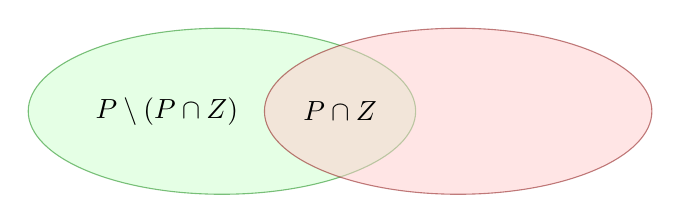
\begin{tikzpicture}
        \filldraw[fill=green!20!white, draw=green!50!black, opacity=0.5] (-1.5,0) ellipse (70pt and 30pt);
        \filldraw[fill=red!20!white, draw=red!50!black, opacity=0.5] (1.5,0) ellipse (70pt and 30pt);
        \node at (0,0) {$P\cap Z$};
        \node at (-2.2,0) {$P\setminus (P\cap Z)$};
    \end{tikzpicture}
    \end{center}

    First check if there are serial or diverging node in $P\cap Z$, if not then check if there are converging node in $P\setminus (P\cap Z)$ and none of the converging node's descendants is in $Z$.

    \textbf{Bascially for a DAG, the other nodes with respect to node $X$ fall into $4$ groups}:

    \begin{center}
    \begin{tikzpicture}
        [nodestyle/.style = {circle,draw=blue!50,fill=blue!20,thick,
                           inner sep=0pt, minimum size=10mm},
         ellinodestyle/.style = {ellipse, draw=blue!50, fill=blue!20, thick,                         minimum width=100pt, align=center},
         outstyle/.style = {-latex'new, arrowhead=0.5cm}]
        \node[nodestyle] (x) at (0,0) {$X$};
        \node[ellinodestyle] (a) at (0,2) {$\it{an}(X)$};
        \node[ellinodestyle] (d) at (0,-2) {$\it{de}(X)$};
        \node[ellinodestyle] (w1) at (-4,0) {$W_1$};
        \node[ellinodestyle] (w2) at (4,0) {$W_2$};
        \draw[outstyle] (a) to (x);
        \draw[outstyle] (x) to (d);
        \draw[outstyle] (a) to (w1);
        \draw[outstyle] (a) to (w2);
        \draw[outstyle] (w2) to (d);
    \end{tikzpicture} 
    \end{center}


\item D-separation: Two nodes $X$ and $Y$ are d-separated by a set $Z$ if all paths between $X$ and $Y$ are blocked by $Z$, $X\perp Y|Z$.

    \textbf{Examples}:

    \begin{tabular}{m{5cm} | m{2cm} | m{5cm} | m{2cm}}
        \hline
        Bayesian Networks & $Z$ separate $X$ and $Y$ ? & Bayesian Networks & $Z$ separate $X$ and $Y$ ?\\ \hline

        \begin{tikzpicture}
            [nodestyle/.style = {circle,draw=blue!50,fill=blue!20,thick,
                               inner sep=0pt, minimum size=5mm},
             outstyle/.style = {-latex'new, arrowhead=0.5cm},
             dotstyle/.style = {circle, fill=cyan!40, inner sep=2pt}]
            \node[nodestyle] (x) at (-1,0) {$X$};
            \node[nodestyle] (y) at (1,0) {$Y$};
            \node[nodestyle] (c) at (0,-1) {};
            \node[nodestyle] (z) at (2,-1) {$Z$};
            \draw[outstyle] (x) to (c);
            \draw[outstyle] (y) to (c);
        \end{tikzpicture} & $\surd$ &
        \begin{tikzpicture}
            [nodestyle/.style = {circle,draw=blue!50,fill=blue!20,thick,
                               inner sep=0pt, minimum size=5mm},
             outstyle/.style = {-latex'new, arrowhead=0.5cm},
             dotstyle/.style = {circle, fill=cyan!40, inner sep=2pt}]
            \node[nodestyle] (x) at (-1,0) {$X$};
            \node[nodestyle] (y) at (1,0) {$Y$};
            \node[nodestyle] (z) at (0,-1) {$Z$};
            \draw[outstyle] (x) to (z);
            \draw[outstyle] (y) to (z);
        \end{tikzpicture} & $\times$\\ \hline 
        \begin{tikzpicture}
            [nodestyle/.style = {circle,draw=blue!50,fill=blue!20,thick,
                               inner sep=0pt, minimum size=5mm},
             outstyle/.style = {-latex'new, arrowhead=0.5cm},
             dotstyle/.style = {circle, fill=cyan!40, inner sep=2pt}]
            \node[nodestyle] (x) at (-1,0) {$X$};
            \node[nodestyle] (y) at (1,0) {$Y$};
            \node[nodestyle] (c) at (0,-1.5) {};
            \node[nodestyle] (z) at (2,-1.5) {$Z$};
            \draw[outstyle] (x) to (c);
            \draw[outstyle] (y) to (c);
            \draw[outstyle] (x) to (z);
            \draw[outstyle] (y) to (z);
        \end{tikzpicture} & $\surd$ & 
        \begin{tikzpicture}
            [nodestyle/.style = {circle,draw=blue!50,fill=blue!20,thick,
                               inner sep=0pt, minimum size=5mm},
             outstyle/.style = {-latex'new, arrowhead=0.5cm},
             dotstyle/.style = {circle, fill=cyan!40, inner sep=2pt}]
            \node[nodestyle] (x) at (-2,0) {$X$};
            \node[nodestyle] (y) at (2,0) {$Y$};
            \node[nodestyle] (c) at (-1,-1) {};
            \node[nodestyle] (d) at (1,-1) {};
            \node[nodestyle] (z) at (0,-2) {$Z$};
            \draw[outstyle] (x) to (c);
            \draw[outstyle] (y) to (d);
            \draw[outstyle] (c) to (z);
            \draw[outstyle] (d) to (z);
        \end{tikzpicture} & $\times$\\ \hline
        \begin{tikzpicture}
            [nodestyle/.style = {circle,draw=blue!50,fill=blue!20,thick,
                               inner sep=0pt, minimum size=5mm},
             outstyle/.style = {-latex'new, arrowhead=0.5cm},
             dotstyle/.style = {circle, fill=cyan!40, inner sep=2pt}]
            \node[nodestyle] (x) at (-1,0) {$X$};
            \node[nodestyle] (y) at (1,0) {$Y$};
            \node[nodestyle] (c) at (0,-1.5) {};
            \node[nodestyle] (d) at (1.5,-1.5) {};
            \node[nodestyle] (e) at (2.5,-1.5) {};
            \node[nodestyle] (f) at (2,-2.5) {};
            \draw[outstyle] (x) to (c);
            \draw[outstyle] (y) to (c);
            \draw[outstyle] (x) to (d);
            \draw[outstyle] (y) to (e);
            \draw[outstyle] (d) to (f);
            \draw[outstyle] (e) to (f);
            \filldraw[fill=green!20!white, draw=green!50!black, opacity=0.8] (2,-2) ellipse (30pt and 30pt);
            \node (z) at (2.7,-2.1) {$Z$};
        \end{tikzpicture} & $\surd$ & 
        \begin{tikzpicture}
            [nodestyle/.style = {circle,draw=blue!50,fill=blue!20,thick,
                               inner sep=0pt, minimum size=5mm},
             outstyle/.style = {-latex'new, arrowhead=0.5cm},
             dotstyle/.style = {circle, fill=cyan!40, inner sep=2pt}]
            \node[nodestyle] (x) at (-2,0) {$X$};
            \node[nodestyle] (y) at (2,0) {$Y$};
            \node[nodestyle] (c) at (-1,-1) {};
            \node[nodestyle] (d) at (1,-1) {};
            \node[nodestyle] (e) at (0,-2) {};
            \draw[outstyle] (x) to (c);
            \draw[outstyle] (y) to (d);
            \draw[outstyle] (c) to (e);
            \draw[outstyle] (d) to (e);
            \filldraw[fill=green!20!white, draw=green!50!black, opacity=0.8] (0,-1.5) ellipse (60pt and 30pt);
            \node (z) at (1.2,-2) {$Z$};
        \end{tikzpicture} & $\surd$\\ \hline  
    \end{tabular}

    \textit{\textbf{Things to note in the examples:} $X$, $Y$ may be dependent or independent, but $X|Z$, $Y|Z$ can be independent so long as they share descendants that are $\notin Z\cup an(Z)$, that's how $Z$ separates $X$ and $Y$.}


\item ancestral set $\it{an}(X)$ of nodes set $X$, $X$ is ancestral if \[X = \it{an}(X)\] 

\item $P_N(X) = P_{N^{'}}(X)$ where $N^{'} = N\setminus Y$, $Y$ is a leaf node of $N$.

\item $P_N(X) = P_{N^{'}}(X)$ where $N^{'} = X$, $X$ is ancestral.

\item Suppose $X$, $Y$, $Z$ are disjoint sets, $X\cup Y\cup Z$ is all the nodes, then $Z$ separates $X$ and $Y$ leads to $X\perp Y|Z$, key is there is no converging node in $Z$ which has parents from both $X$ and $Y$, otherwise the length-2 path with 1 parent from $X$ and the other from $Y$ is not separated by $Z$.

\item Global Markov property: variables $X$ and $Y$, $X\perp Y|Z$ if $X\notin Z$, $Y\notin Z$, and $Z$ separates them. \[ \mathcal{S_G}(X,Y,Z) \Rightarrow X\perp_{P} Y|Z \]

\item Markov blanket: (parents + children + parents of children) of node $X$.

\item Local Markov property: given parents, variable $X$ is independent of all its non-descendants. \[ X\perp_{P} \it{nd}_\mathcal{G}(X)|\it{pa}_\mathcal{G}(X) \]

\item $\mathcal{G}$ to $P(V)$ is called \textbf{\color{cyan}I-map}: $\mathcal{S_G}(X,Y,Z) \Rightarrow X\perp_{P} Y|Z$, \textbf{\color{cyan}D-map}: $X\perp_{P} Y|Z \Rightarrow \mathcal{S_G}(X,Y,Z)$, \textbf{\color{cyan}Perfect map}: $\mathcal{S_G}(X,Y,Z) \Leftrightarrow X\perp_{P} Y|Z$.
\end{itemize}
